%
%  Name: Labelled Transition System
%  For: obsidian notes
%  Created: 2025-10-03
%
\documentclass{standalone}
\usepackage{amsmath}
\usepackage{tikz}
\usetikzlibrary{arrows,automata,positioning}

\usepackage{xcolor}
\definecolor{halcyon-base-blue-01}{HTML}{171c28}    % Workbench Background
\definecolor{halcyon-base-blue-01}{HTML}{1d2433}    % Editor Background
\definecolor{halcyon-base-blue-03}{HTML}{2f3b54}    % Highlight, widgets, panel
\definecolor{halcyon-base-blue-04}{HTML}{6679a4}    % Dividers, subtle UI elements
\definecolor{halcyon-base-blue-05}{HTML}{8695b7}    % Status bar text, buttons, etc.
\definecolor{halcyon-base-grey-dark}{HTML}{a2aabc}  % Variables, property names, tabs
\definecolor{halcyon-base-grey-light}{HTML}{d7dce2} % Active text, anything that should be white

\definecolor{halcyon-accent}{HTML}{ffcc66}          % Accent, list tree titles, badges, etc.

\definecolor{halcyon-palette-cyan}{HTML}{5ccfe6}    % - UI: Modified highlights
\definecolor{halcyon-palette-lime}{HTML}{bae67e}    % - UI: Addition highlights
\definecolor{halcyon-palette-orange}{HTML}{ffae57}  % Constants, operators
\definecolor{halcyon-palette-yellow}{HTML}{ffd580}  % Functions, classes, object literal keys
\definecolor{halcyon-palette-lilac}{HTML}{c3a6ff}   % Keywords, constants, template literals
\definecolor{halcyon-palette-salmon}{HTML}{ef6b73}  % Deletion highlights, errors, warnings

\begin{document}

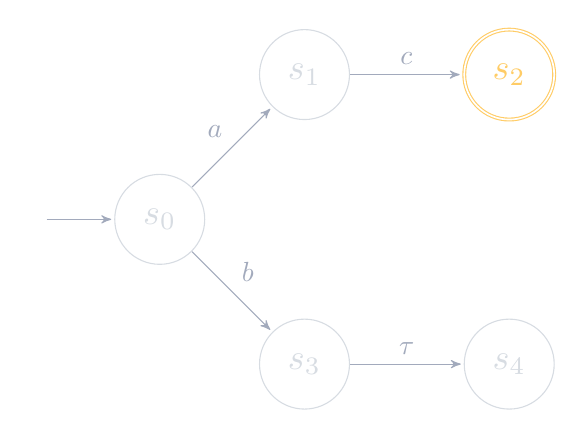
\begin{tikzpicture}[>=stealth', shorten >=1pt,node distance=2cm,auto]
  \tikzstyle{every state}=[style={scale=1.3},halcyon-base-grey-light]

  \node        (l1) {};
  \node[state]            (s0) [right of=l1, xshift=-8mm]  {$s_0$};
  \node[state]            (s1) [above right of=s0]         {$s_1$};
  \node[state, accepting, halcyon-accent] (s2) [right of=s1]               {$s_2$};
  \node[state]            (s3) [below right of=s0]         {$s_3$};
  \node[state]            (s4) [right of=s3]               {$s_4$};

  %% L1 path
  \path[->,halcyon-base-grey-dark]
  (l1)  edge node {}    (s0)
  (s0)  edge node {$a$} (s1)
  (s1)  edge node {$c$} (s2)

  (s0)  edge node {$b$} (s3)
  (s3)  edge node {$\tau$} (s4);
\end{tikzpicture}
\end{document}